\chapter{Evaluation}
\label{ch:eval}
In this chapter, experiments are conducted to evaluate the correctness and performance of k8-resource-optimizer in Chapter~\ref{ch:eval}. The first experiment validates the correctness of the employed workload generator. The second experiment validates the CPU dependency of the application. The remainder of the experiments validate the SLA-decomposition capabilities of k8-resource-optimizer in various settings.

\section{Evaluation environment}
The experiments in this chapter are conducted on a single-node Kubernetes cluster (version 1.8.0) inside a VM using Minikube~\cite{minikube-web} (version 0.24.1). The VM is allocated 4 cores and 8192 MB memory. The underlying hardware utilizes a 2.6GHz hyper-threading quad-core processor.  

%%%%%%%%%%%%%%%
% EXPERIMENT 1
%%%%%%%%%%%%%%%

\section{Experiment 1: Workload generator validation}
The k8-resource-optimizer tool (Section~\ref{ch:k8-bench}) uses Locust (Section~\ref{locust-wrapper}) as a workload generator to evaluate the performance of an application. Section~\ref{sec:little} showed that Little's law can be used to evaluate the correctness of such a load testing tool. Since the benchmark is a key component for the tool, an experiment is conducted to check its correctness (i.e., it generates the correct amount of concurrent users). 
\paragraph{Experiment setup} 
For the experiment two Kubernetes namespaces, large and small, are created on the cluster. In both namespaces  an instance of the simple batch processing application is deployed. The CPU quota for the worker pod in the large and small namespace are respectively set to 500 Millicores and 250 Millicores. This refers to both limit and request settings. The size of jobs submitted to the queues by tenants of big and small is 1000 tasks. In three consecutive runs different amounts of each user-type are created. 
\paragraph{Results}
The results generated by Locust are shown in Table~\ref{tab:locust}. Little's law states that $\textit{average response time} * \textit{throughput} = \textit{concurrent amount of users}$. This is shown in the last column. The first column shows the amount of specified users. The results show that concurrency for each user-type generated by Locust is close to the specified amount. As, such it can be concluded that Locust is a valid workload generation tool.
\begin{table}[H]
\caption {Experiment 1: Results Little's law based evaluation of workload generation tool. The amount of concurrency is close to the requested amount of users.} \label{tab:locust} 
\begin{tabular}{llllll}
\hline
\multicolumn{1}{|l|}{\textbf{\# users}}  & \multicolumn{1}{l|}{\textbf{Name}} & \multicolumn{1}{l|}{\textbf{\# requests}} & \multicolumn{1}{l|}{\textbf{Average RT}} & \multicolumn{1}{l|}{\textbf{Requests/s}} & \multicolumn{1}{l|}{\textbf{Concurrent users}} \\ \hline
\multicolumn{1}{|l|}{1}                  & \multicolumn{1}{l|}{large}          & \multicolumn{1}{l|}{128}                  & \multicolumn{1}{l|}{2930}                & \multicolumn{1}{l|}{0.34}                & \multicolumn{1}{l|}{1.02}                      \\ \hline
\multicolumn{1}{|l|}{1}                  & \multicolumn{1}{l|}{small}        & \multicolumn{1}{l|}{73}                   & \multicolumn{1}{l|}{5163}                & \multicolumn{1}{l|}{0.19}                & \multicolumn{1}{l|}{0.98097}                   \\ \hline
\multicolumn{1}{|l|}{2}                  & \multicolumn{1}{l|}{total}         & \multicolumn{1}{l|}{201}                  & \multicolumn{1}{l|}{3741}                & \multicolumn{1}{l|}{0.54}                & \multicolumn{1}{l|}{2.02014}                   \\ \hline
                                         &                                    &                                           &                                          &                                          &                                                \\ \hline
\multicolumn{1}{|l|}{\textbf{\# users}}  & \multicolumn{1}{l|}{\textbf{Name}} & \multicolumn{1}{l|}{\textbf{\# requests}} & \multicolumn{1}{l|}{\textbf{Average RT}} & \multicolumn{1}{l|}{\textbf{Requests/s}} & \multicolumn{1}{l|}{\textbf{Concurrent users}} \\ \hline
\multicolumn{1}{|l|}{2}                  & \multicolumn{1}{l|}{large}          & \multicolumn{1}{l|}{275}                  & \multicolumn{1}{l|}{4806}                & \multicolumn{1}{l|}{0.41}                & \multicolumn{1}{l|}{1.97046}                   \\ \hline
\multicolumn{1}{|l|}{2}                  & \multicolumn{1}{l|}{small}        & \multicolumn{1}{l|}{128}                  & \multicolumn{1}{l|}{10360}               & \multicolumn{1}{l|}{0.19}                & \multicolumn{1}{l|}{1.9684}                    \\ \hline
\multicolumn{1}{|l|}{4}                  & \multicolumn{1}{l|}{total}         & \multicolumn{1}{l|}{403}                  & \multicolumn{1}{l|}{6570}                & \multicolumn{1}{l|}{0.61}                & \multicolumn{1}{l|}{4.0077}                    \\ \hline
                                         &                                    &                                           &                                          &                                          &                                                \\ \hline
\multicolumn{1}{|l|}{\textbf{\#  users}} & \multicolumn{1}{l|}{\textbf{Name}} & \multicolumn{1}{l|}{\textbf{\# requests}} & \multicolumn{1}{l|}{\textbf{Average RT}} & \multicolumn{1}{l|}{\textbf{Requests/s}} & \multicolumn{1}{l|}{\textbf{Concurrent users}} \\ \hline
\multicolumn{1}{|l|}{3}                  & \multicolumn{1}{l|}{large}          & \multicolumn{1}{l|}{279}                  & \multicolumn{1}{l|}{7127}                & \multicolumn{1}{l|}{0.42}                & \multicolumn{1}{l|}{2.99334}                   \\ \hline
\multicolumn{1}{|l|}{1}                  & \multicolumn{1}{l|}{small}        & \multicolumn{1}{l|}{124}                  & \multicolumn{1}{l|}{5340}                & \multicolumn{1}{l|}{0.19}                & \multicolumn{1}{l|}{1.0146}                    \\ \hline
\multicolumn{1}{|l|}{4}                  & \multicolumn{1}{l|}{total}         & \multicolumn{1}{l|}{403}                  & \multicolumn{1}{l|}{6577}                & \multicolumn{1}{l|}{0.61}                & \multicolumn{1}{l|}{4.01197}                   \\ \hline
\end{tabular}
\end{table}


%%%%%%%%%%%%%%%
% EXPERIMENT 2
%%%%%%%%%%%%%%%
\section{Experiment 2: Effect of job size and tenant concurrency on throughput}
Chapter~\ref{chapter_app} describes the application used to evaluate the k8-resource-optimizer tool. The application accepts jobs containing a variable amount of tasks. The maximum size of a job is an integral part of a tenant's SLO specification. The purpose of the following experiment is to validate that a job size influences the performance of an application. In addition, the experiment inspects the impact of multiple concurrent tenants on the throughput. 

\paragraph{Experiment setup}
In the experiment a single Kubernetes namespace is created on the cluster, in which  an instance of the  application is deployed. In other words, there a single queue and worker are deployed. The CPU request and limit for the worker pod is set to 1000 Millicores. The complete experiment consists out of two sub-experiments. In each sub-experiment multiple iterations of Locust experiments are executed. During the iterations the job size is increased from 100 to 2900 tasks in steps of 100 tasks. In the first sub-experiment, a single tenant submits 50 successive jobs to the application each iteration.  In the second sub-experiment, a total of 100 jobs are submitted in each iteration by two concurrent tenants. Separately, the sub-experiments provide insights into the effect of the job size on the performance of the application. Combined the experiments show how the performance of the application varies in the presence of concurrent tenants.  


\paragraph{Results}
The results of both sub-experiments are shown in Figure~\ref{fig:exp2B-jobsize}. As expected an increasing job size results in a lower throughput. The Locust experiments with two concurrent tenants achieve an overall higher throughput compared to those of a single tenant. This a consequence of the inner workings of the tested application. By utilizing a pull queue, a worker must periodically poll the queue for tasks. Each poll starts a new thread. When a thread is finished executing a task, it will acknowledge that task and immediately check for a new task. Hence, multiple threads can be started. With a single tenant, the queue is empty between jobs. This results in worker threads to be stopped. This is not the case in the presence of multiple tenants. As a consequence, Figure~\ref{fig:jobsizegrafana} shows that two tenants utilize more CPU compared to a single tenant. It also shows that the worker pod is only capable of using 750 of 1000 Millicores. This indicates that vertical scaling of the worker beyond 750 Millicores probably has no positive effect on its performance.

\begin{figure}[H]
    \centering
    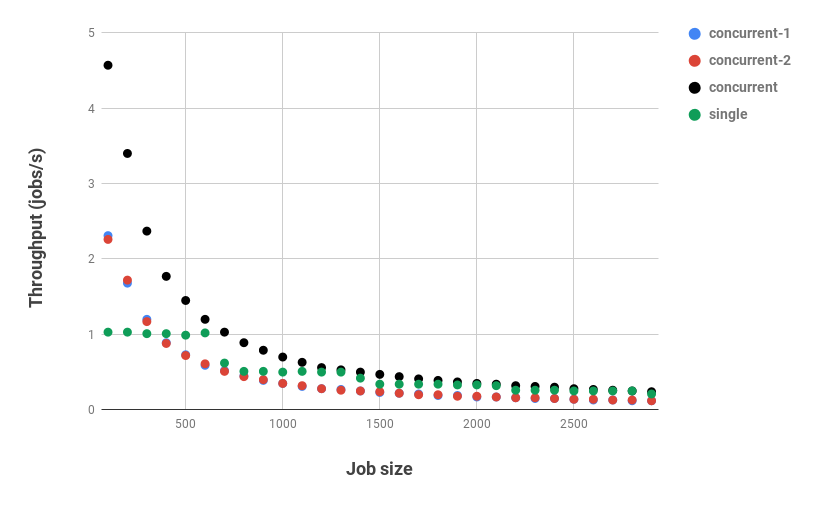
\includegraphics[width=1\textwidth]{chapter-evaluation/jobsize-cpu.png}
    \caption{Experiment 2: Influence of job size and  user concurrency on throughput. }
    \label{fig:exp2B-jobsize}
\end{figure}
\begin{figure}[H]
\centering
\subfigure[Single tenant.]{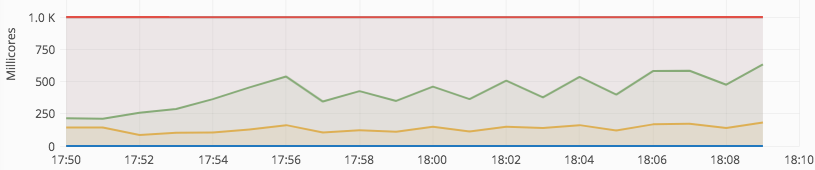
\includegraphics[width=0.9\linewidth]{chapter-evaluation/jobsize.png}\label{jobsize:sub1}}
\subfigure[Two tenants.]{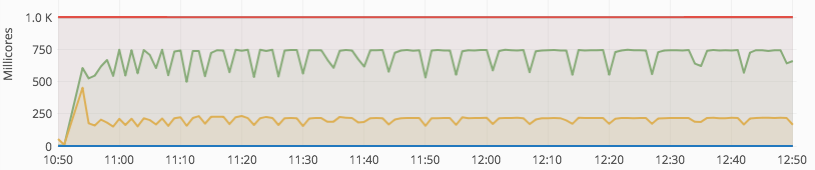
\includegraphics[width=0.9\linewidth]{chapter-evaluation/jobsize-concurrent.png}\label{jobsize:sub2}}
\caption{Experiment 2: Grafana dashboard CPU utilization. }
\label{fig:jobsizegrafana}
\end{figure}


%%%%%%%%%%%%%%%
% EXPERIMENT 3
%%%%%%%%%%%%%%%
\section{Experiment 3: Single SLA  single parameter}
The goal of this experiment is to test the auto-tune capability of k8-resource-optimizer for a single configuration parameter of a single tenant. The parameter under tune is the CPU resource limit and request for the worker component of the application. This parameter will be referred to as \texttt{workerCPU} for the remainder of this chapter. The objective is to find a minimum configuration setting that satisfies the SLA.
\begin{figure}[H]
    \centering
    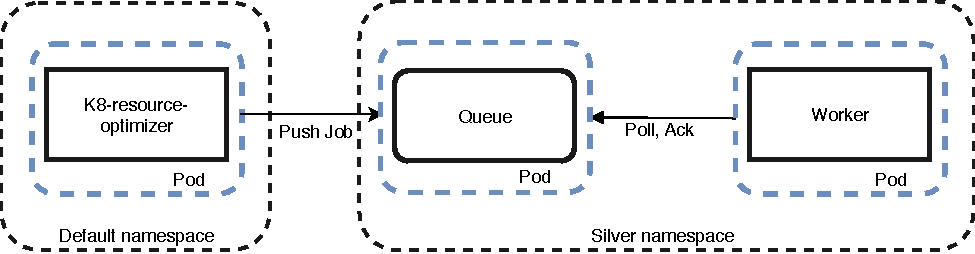
\includegraphics[width=0.7\textwidth]{chapter-evaluation/experiment-2-deployment.pdf}
    \caption{Experiment 3: Deployment single SLA single parameter.}
    \label{fig:exp2-deployment}
\end{figure}

\paragraph{Experiment setup}
The k8-resource-optimizer input configuration for the experiment is shown in Listing~\ref{lst:exp2-config}.
k8-resource-optimizer will optimize the  application for a single tenant of the silver SLA-class. This class requires a minimum throughput of 0.5 jobs per second where each job contains up to 500 tasks. To test whether a configuration meets the SLO, each configuration is load tested with three Locust experiments. One experiment for each of the following job sizes:  300, 400 or 500 tasks. Every experiment performs 10 warm-up request and 50 measured requests. This is to cope with the presence of a cold start. The search space for parameter \texttt{workerCPU} is between 200 Millicores and 1000 Millicores. The optimization will perform 4 iterations of \textit{DDS} and \textit{RBS} ( Section~\ref{rw:bestconfig}). Each iteration tests 4 configuration samples. Resulting in  16 configurations to be tested in total.  Figure~\ref{fig:exp2-deployment} illustrates the deployment of the experiment in the cluster. The tool itself is also deployment inside a pod in the cluster.



\begin{lstlisting}[caption=Experiment 3: Input configuration., language=yaml, label={lst:exp2-config}]
---
iterations: 4
samples: 4
charts:
  - name: my-app
    chartdir: /exp/conf/helm/mychart
slas:
  - name : silver
    chart: my-app
    jobsize: 500
    throughput: 0.5
    amount: 1
    parameters:
      - name: workerCPU
        searchspace:
          min: 200
          max: 1000
        prefix: 
        suffix: m
strategy: NSPSLA

---
\end{lstlisting}
\paragraph{Results}
The results of the experiment produced by k8-resource-optimizer are shown in Table~\ref{tbl:results2}. These results show that samples picked by the tool during the first iteration provide a wide coverage of the search space. Configuration samples assigned a zero score do not meet the required SLO. The throughput shown is for the largest experiment with job size 500. During each next iteration, a narrower search space is selected by \textit{RBS} as expected. This is visible in Figure~\ref{fig:exp2-results} as the density of samples is the highest between 345 and 400. A CPU resource and limit setting of 360 is the most optimal found by the tool in 4 iterations. Table~\ref{tbl:exp2-increase} shows the increase of the best score after each iteration. This shows that the second iteration provides a much larger increase compared to the later iterations. \\
\par 
\noindent The total execution of the experiment took approximately 2 hours and 10 minutes as shown in Figure~\ref{fig:exp2-grafana}. The majority of the time is spent executing the load tests. Depending on the impact of a 3\% (in this case) more cost-efficient setup in a production environment the later iterations could be discarded.


\begin{figure}[H]
    \centering
    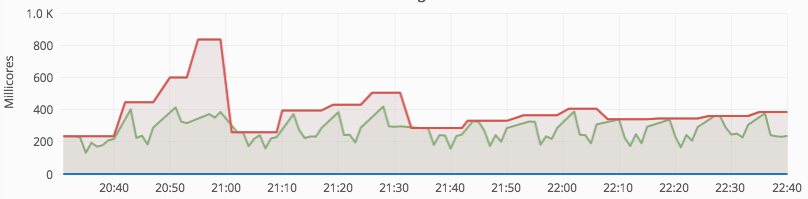
\includegraphics[width=1\textwidth]{chapter-evaluation/single-sla-2-granfana.png}
    \caption{Experiment 3: Metrics Grafana dashboard. }
    \label{fig:exp2-grafana}
\end{figure}



\begin{table}[H]
\caption{Experiment 3: Results of k8-resource-optimizer on 16 samples in 4 iterations.}
\label{tbl:results2}
\centering
\begin{tabular}{lll}
ITERATION: 1                             &                                     &                                                  \\ \hline
\multicolumn{1}{|l|}{\textbf{workerCPU}} & \multicolumn{1}{l|}{\textbf{Score}} & \multicolumn{1}{l|}{\textbf{Throughput on 500 tasks (Jobs/s)}} \\ \hline
\multicolumn{1}{|l|}{235}                & \multicolumn{1}{l|}{0}              & \multicolumn{1}{l|}{0.34}                        \\ \hline
\multicolumn{1}{|l|}{445}                & \multicolumn{1}{l|}{2.25}           & \multicolumn{1}{l|}{0.52}                        \\ \hline
\multicolumn{1}{|l|}{600}                & \multicolumn{1}{l|}{1.67}           & \multicolumn{1}{l|}{0.95}                        \\ \hline
\multicolumn{1}{|l|}{835}                & \multicolumn{1}{l|}{1.2}            & \multicolumn{1}{l|}{1.01}                        \\ \hline
                                         &                                     &                                                  \\
ITERATION: 2                             &                                     &                                                  \\ \hline
\multicolumn{1}{|l|}{\textbf{workerCPU}} & \multicolumn{1}{l|}{\textbf{Score}} & \multicolumn{1}{l|}{\textbf{Throughput on 500 tasks (Jobs/s)}} \\ \hline
\multicolumn{1}{|l|}{260}                & \multicolumn{1}{l|}{0}              & \multicolumn{1}{l|}{0.37}                        \\ \hline
\multicolumn{1}{|l|}{380}                & \multicolumn{1}{l|}{2.63}           & \multicolumn{1}{l|}{0.51}                        \\ \hline
\multicolumn{1}{|l|}{450}                & \multicolumn{1}{l|}{2.22}           & \multicolumn{1}{l|}{0.52}                        \\ \hline
\multicolumn{1}{|l|}{560}                & \multicolumn{1}{l|}{1.79}           & \multicolumn{1}{l|}{0.54}                        \\ \hline
                                         &                                     &                                                  \\
ITERATION: 3                             &                                     &                                                  \\ \hline
\multicolumn{1}{|l|}{\textbf{workerCPU}} & \multicolumn{1}{l|}{\textbf{Score}} & \multicolumn{1}{l|}{\textbf{Throughput on 500 tasks (Jobs/s)}} \\ \hline
\multicolumn{1}{|l|}{275}                & \multicolumn{1}{l|}{0}              & \multicolumn{1}{l|}{0.39}                        \\ \hline
\multicolumn{1}{|l|}{345}                & \multicolumn{1}{l|}{0}              & \multicolumn{1}{l|}{0.48}                        \\ \hline
\multicolumn{1}{|l|}{370}                & \multicolumn{1}{l|}{2.7}            & \multicolumn{1}{l|}{0.51}                        \\ \hline
\multicolumn{1}{|l|}{395}                & \multicolumn{1}{l|}{2.53}           & \multicolumn{1}{l|}{0.53}                        \\ \hline
                                         &                                     &                                                  \\
ITERATION: 4                             &                                     &                                                  \\ \hline
\multicolumn{1}{|l|}{\textbf{workerCPU}} & \multicolumn{1}{l|}{\textbf{Score}} & \multicolumn{1}{l|}{\textbf{Throughput on 500 tasks (Jobs/s)}} \\ \hline
\multicolumn{1}{|l|}{350}                & \multicolumn{1}{l|}{0}              & \multicolumn{1}{l|}{0.48}                        \\ \hline
\multicolumn{1}{|l|}{360}                & \multicolumn{1}{l|}{2.78}           & \multicolumn{1}{l|}{0.5}                         \\ \hline
\multicolumn{1}{|l|}{365}                & \multicolumn{1}{l|}{2.74}           & \multicolumn{1}{l|}{0.5}                         \\ \hline
\multicolumn{1}{|l|}{375}                & \multicolumn{1}{l|}{2.67}           & \multicolumn{1}{l|}{0.52}                        \\ \hline
\end{tabular}
\end{table}


\begin{figure}[H]
    \centering
    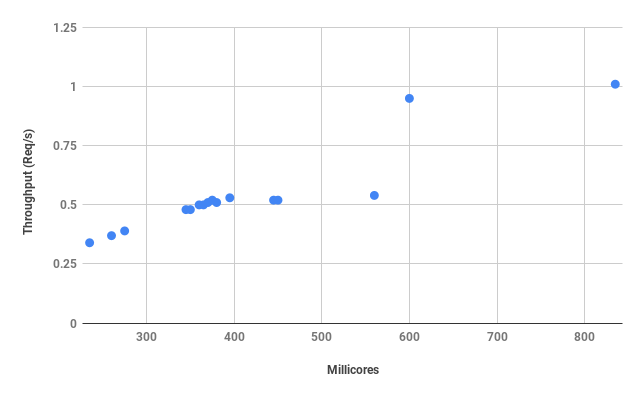
\includegraphics[width=1\textwidth]{chapter-evaluation/exp2-results-2.png}
    \caption{Experiment 2: Throughput vs. CPU sample results   }
    \label{fig:exp2-results}
\end{figure}

\begin{table}[H]
\caption{Experiment 3: Utility function score increase per iteration in percentage.}
\label{tbl:exp2-increase}
\centering
\begin{tabular}{|l|l|l|}
\hline
\textbf{Iteration} & \textbf{Best score} & \textbf{Increase \%} \\ \hline
0                  & 2.25                & 0                    \\ \hline
1                  & 2.63                & 17                   \\ \hline
2                  & 2.7                 & 3                    \\ \hline
3                  & 2.78                & 3                    \\ \hline
\end{tabular}
\end{table}





%%%%%%%%%%%%%%%
% EXPERIMENT 4
%%%%%%%%%%%%%%%
\newpage
\section{Experiment 4: Set of tenants with homogeneous SLA classes}
The following  experiment is conducted in order to evaluate the capability of k8-resource-optimizer to perform a SLA-decomposition for multiple tenants of the same SLA class. The parameter under tune is \texttt{workerCPU}.  The experiment utilizes the shared namespace per SLA class strategy to achieve multi-tenancy within Kubernetes as discussed in Section~\ref{rw:eddy}. 

\paragraph{Experiment setup}
For this experiment a SLA-decomposition is conducted for two silver tenants. The SLO of the silver SLA class is the same as in Experiment 3. In the shared namespace per SLA class strategy, both tenants send requests to the same application instance running in a single Kubernetes namespace.  Similar to Experiment 3,  three separate Locust experiments are conducted. Since two concurrent tenants are present the Locust experiments perform a total of 100 measured requests. In each experiment, Locust will spawn two users. The SLO must be met for each user separately.  The search space for the parameter \texttt{workerCPU} is between 200 Millicores and 800 Millicores. The optimization will perform 3 iterations of \textit{DDS} and \textit{RBS} ( Section~\ref{rw:bestconfig}). Each iteration tests 4 configuration samples. Resulting in  12 configurations to be tested in total.  The deployment of the namespace per SLA class strategy is the same as illustrated in Figure~\ref{fig:exp2-deployment}. 

\paragraph{Results}
The results of the experiment produced by k8-resource-optimizer are shown in Table~\ref{tbl:results4}.  The best CPU setting for the worker pod found to support two tenants is 560 Millicores. Compared with 360 Millicores for a single tenant in  the previous experiment, it shows that the application performance does not scale linearly with the CPU setting. Table~\ref{tbl:exp4-increase} shows the best score increase in percentage for each iteration. In the last iteration, no better setting is found. If a fourth iteration was executed a backtrack step to the second search space would be performed. The execution of the experiment took approximately 1 hour and 30 minutes. The overall results show that k-bench has the capability to auto-tune for multiple tenants.
\begin{table}[H]
\centering
\caption{Experiment 4: Namespace per SLA utility function score increase per iteration in percentage.}
\label{tbl:exp4-increase}
\begin{tabular}{|l|l|l|}
\hline
\textbf{Iteration} & \textbf{Best score} & \textbf{Increase \%} \\ \hline
0                  & 1.39                & 0                    \\ \hline
1                  & 1.43                & 3                    \\ \hline
2                  & 1.38                & -3                   \\ \hline
\end{tabular}
\end{table}

\begin{table}[H]
\centering
\caption{Experiment 4: Namespace per SLA results of k8-resource-optimizer on 12 samples in 3 iterations. Throughput is for job size of 500 tasks.}
\label{tbl:results4}
\begin{tabular}{llll}
ITERATION: 1                             &                                     &                                                 &                                                 \\ \hline
\multicolumn{1}{|l|}{\textbf{workerCPU}} & \multicolumn{1}{l|}{\textbf{Score}} & \multicolumn{1}{l|}{\textbf{Tenant 1  (Jobs/s)}} & \multicolumn{1}{l|}{\textbf{Tenant 2  (Jobs/s)}} \\ \hline
\multicolumn{1}{|l|}{335}                & \multicolumn{1}{l|}{0}              & \multicolumn{1}{l|}{0.28}                       & \multicolumn{1}{l|}{0.27}                       \\ \hline
\multicolumn{1}{|l|}{545}                & \multicolumn{1}{l|}{0}              & \multicolumn{1}{l|}{0.49}                       & \multicolumn{1}{l|}{0.48}                       \\ \hline
\multicolumn{1}{|l|}{575}                & \multicolumn{1}{l|}{1.39}           & \multicolumn{1}{l|}{0.53}                       & \multicolumn{1}{l|}{0.52}                       \\ \hline
\multicolumn{1}{|l|}{735}                & \multicolumn{1}{l|}{1.09}           & \multicolumn{1}{l|}{0.64}                       & \multicolumn{1}{l|}{0.65}                       \\ \hline
                                         &                                     &                                                 &                                                 \\
ITERATION: 2                             &                                     &                                                 &                                                 \\ \hline
\multicolumn{1}{|l|}{\textbf{workerCPU}} & \multicolumn{1}{l|}{\textbf{Score}} & \multicolumn{1}{l|}{\textbf{Tenant 1 (Jobs/s)}}   & \multicolumn{1}{l|}{\textbf{Tenant 2 (Jobs/s)}}  \\ \hline
\multicolumn{1}{|l|}{560}                & \multicolumn{1}{l|}{1.43}           & \multicolumn{1}{l|}{0.52}                       & \multicolumn{1}{l|}{0.51}                       \\ \hline
\multicolumn{1}{|l|}{630}                & \multicolumn{1}{l|}{1.27}           & \multicolumn{1}{l|}{0.59}                       & \multicolumn{1}{l|}{0.6}                        \\ \hline
\multicolumn{1}{|l|}{655}                & \multicolumn{1}{l|}{1.22}           & \multicolumn{1}{l|}{0.61}                       & \multicolumn{1}{l|}{0.62}                       \\ \hline
\multicolumn{1}{|l|}{680}                & \multicolumn{1}{l|}{1.18}           & \multicolumn{1}{l|}{0.63}                       & \multicolumn{1}{l|}{0.64}                       \\ \hline
                                         &                                     &                                                 &                                                 \\
ITERATION: 3                             &                                     &                                                 &                                                 \\ \hline
\multicolumn{1}{|l|}{\textbf{workerCPU}} & \multicolumn{1}{l|}{\textbf{Score}} & \multicolumn{1}{l|}{\textbf{Tenant 1  (Jobs/s)}} & \multicolumn{1}{l|}{\textbf{Tenant 2  (Jobs/s)}} \\ \hline
\multicolumn{1}{|l|}{555}                & \multicolumn{1}{l|}{0}              & \multicolumn{1}{l|}{0.49}                       & \multicolumn{1}{l|}{0.49}                       \\ \hline
\multicolumn{1}{|l|}{580}                & \multicolumn{1}{l|}{1.38}           & \multicolumn{1}{l|}{0.51}                       & \multicolumn{1}{l|}{0.5}                        \\ \hline
\multicolumn{1}{|l|}{595}                & \multicolumn{1}{l|}{1.34}           & \multicolumn{1}{l|}{0.56}                       & \multicolumn{1}{l|}{0.55}                       \\ \hline
\multicolumn{1}{|l|}{615}                & \multicolumn{1}{l|}{1.3}            & \multicolumn{1}{l|}{0.59}                       & \multicolumn{1}{l|}{0.57}                       \\ \hline
\end{tabular}
\end{table}


% \paragraph{Results namespace per tenant}
% In the namespace per tenant strategy, both tenants send requests to different application instances running in separate Kubernetes namespaces. Both instances (namespaces) are simultaneously tuned by k8-resource-optimizer.


%%%%%%%%%%%%%%%
% EXPERIMENT 5
%%%%%%%%%%%%%%%
\section{Experiment 5:  Mix of tenants with heterogeneous SLA classes}
The goal of the following experiment is the auto-tune capability of k8-resource-optimizer for a mix of tenants with different SLA classes. The parameter under tune is \texttt{workerCPU}. The namespace per SLA class strategy is used.
\paragraph{Experiment setup}
For this experiment, a SLA-decomposition is performed for a single silver and a single bronze tenant. The SLO specifications for the silver SLA class are the same as in Experiment 2. The bronze SLA class requires a minimum throughput of 0.5 jobs per second where each job contains up to 250 tasks. \\
During the experiment, two instance of the application are deployed in two separate namespaces. The worker CPU parameter for both instances is tuned simultaneously. The search space the \texttt{workerCPU} for the silver and bronze namespace are respectively \texttt{200 - 800} and \texttt{100 - 700}. The optimization will perform 3 iterations of \textit{DDS} and \textit{RBS}. Each iteration tests 4 configurations samples (pair of silver and bronze setting). Resulting in  12 configurations to be tested in total.\\
To test whether the configurations meet their required SLOs, three Locust experiments are conducted on each sample . In each experiment, two Locust users are concurrently spawned and executed. One for each type of tenant. During the three Locust experiments the job size is increased in steps of 100 tasks, starting from 300 tasks for silver and 50 tasks for bronze. In total each experiment performs 150 requests. 

\paragraph{Results}
The results of the experiment produced by k8-resource-optimizer are shown in Table~\ref{tbl:results-5}. The best \texttt{WorkerCPU} settings found for bronze and silver are respectively 225 Millicores and 360 Millicores. The increase in best score for each SLA is shown Table~\ref{tbl:exp5-increase}. For the silver namespace no better is found within search space \texttt{290 - 600} during the second iteration. Therefore, a backtrack to the original namespace is performed during the last iteration. However, the setting with the best score found during the last iteration is within that second search space. This is an example in which backtracking might be performed prematurely. The execution of the experiment took approximately 1 hour and 30 minutes.  The overall results indicate that k8-resource-optimizer is capable of tuning multiple namespaces simultaneously.



\begin{table}[H]
\caption{Experiment 5: Results of k8-resource-optimizer on 12 samples in 3 iterations for mix of bronze and silver tenants. Throughput is for job size of 250  tasks for bronze and 500 tasks for silver.}
\label{tbl:results-5}
\centering
\begin{tabular}{lllllll}
\textbf{Bronze}                          & \textbf{}                           & \textbf{}                             & \textbf{}                      & \textbf{Silver}                         & \textbf{}                           & \textbf{}                             \\
                                         &                                     &                                       &                                &                                         &                                     &                                       \\
ITERATION: 1                             &                                     &                                       &                                & ITERATION: 1                            &                                     &                                       \\ \cline{1-3} \cline{5-7} 
\multicolumn{1}{|l|}{\textbf{workerCPU}} & \multicolumn{1}{l|}{\textbf{Score}} & \multicolumn{1}{l|}{\textbf{(Jobs/s)}} & \multicolumn{1}{l|}{\textbf{}} & \multicolumn{1}{l|}{\textbf{workerCPU}} & \multicolumn{1}{l|}{\textbf{Score}} & \multicolumn{1}{l|}{\textbf{(Jobs/s)}} \\ \cline{1-3} \cline{5-7} 
\multicolumn{1}{|l|}{205}                & \multicolumn{1}{l|}{0}              & \multicolumn{1}{l|}{0.48}             & \multicolumn{1}{l|}{}          & \multicolumn{1}{l|}{290}                & \multicolumn{1}{l|}{0}              & \multicolumn{1}{l|}{0.35}             \\ \cline{1-3} \cline{5-7} 
\multicolumn{1}{|l|}{655}                & \multicolumn{1}{l|}{1.07}           & \multicolumn{1}{l|}{1}                & \multicolumn{1}{l|}{}          & \multicolumn{1}{l|}{390}                & \multicolumn{1}{l|}{2.05}           & \multicolumn{1}{l|}{0.51}             \\ \cline{1-3} \cline{5-7} 
\multicolumn{1}{|l|}{480}                & \multicolumn{1}{l|}{1.46}           & \multicolumn{1}{l|}{1.01}             & \multicolumn{1}{l|}{}          & \multicolumn{1}{l|}{600}                & \multicolumn{1}{l|}{1.33}           & \multicolumn{1}{l|}{0.63}             \\ \cline{1-3} \cline{5-7} 
\multicolumn{1}{|l|}{270}                & \multicolumn{1}{l|}{2.59}           & \multicolumn{1}{l|}{0.53}             & \multicolumn{1}{l|}{}          & \multicolumn{1}{l|}{655}                & \multicolumn{1}{l|}{1.22}           & \multicolumn{1}{l|}{0.95}             \\ \cline{1-3} \cline{5-7} 
                                         &                                     &                                       &                                &                                         &                                     &                                       \\
ITERATION: 2                             &                                     &                                       &                                & ITERATION: 2                            &                                     &                                       \\ \cline{1-3} \cline{5-7} 
\multicolumn{1}{|l|}{\textbf{workerCPU}} & \multicolumn{1}{l|}{\textbf{Score}} & \multicolumn{1}{l|}{\textbf{(Jobs/s)}} & \multicolumn{1}{l|}{\textbf{}} & \multicolumn{1}{l|}{\textbf{workerCPU}} & \multicolumn{1}{l|}{\textbf{Score}} & \multicolumn{1}{l|}{\textbf{(Jobs/s)}} \\ \cline{1-3} \cline{5-7} 
\multicolumn{1}{|l|}{370}                & \multicolumn{1}{l|}{1.89}           & \multicolumn{1}{l|}{0.93}             & \multicolumn{1}{l|}{}          & \multicolumn{1}{l|}{435}                & \multicolumn{1}{l|}{1.84}           & \multicolumn{1}{l|}{0.5}              \\ \cline{1-3} \cline{5-7} 
\multicolumn{1}{|l|}{420}                & \multicolumn{1}{l|}{1.67}           & \multicolumn{1}{l|}{1}                & \multicolumn{1}{l|}{}          & \multicolumn{1}{l|}{325}                & \multicolumn{1}{l|}{0}              & \multicolumn{1}{l|}{0.39}             \\ \cline{1-3} \cline{5-7} 
\multicolumn{1}{|l|}{245}                & \multicolumn{1}{l|}{2.86}           & \multicolumn{1}{l|}{0.51}             & \multicolumn{1}{l|}{}          & \multicolumn{1}{l|}{515}                & \multicolumn{1}{l|}{1.55}           & \multicolumn{1}{l|}{0.52}             \\ \cline{1-3} \cline{5-7} 
\multicolumn{1}{|l|}{325}                & \multicolumn{1}{l|}{2.15}           & \multicolumn{1}{l|}{0.56}             & \multicolumn{1}{l|}{}          & \multicolumn{1}{l|}{440}                & \multicolumn{1}{l|}{1.82}           & \multicolumn{1}{l|}{0.52}             \\ \cline{1-3} \cline{5-7} 
                                         &                                     &                                       &                                &                                         &                                     &                                       \\
ITERATION: 3                             &                                     &                                       &                                & ITERATION: 3                            &                                     &                                       \\ \cline{1-3} \cline{5-7} 
\multicolumn{1}{|l|}{\textbf{workerCPU}} & \multicolumn{1}{l|}{\textbf{Score}} & \multicolumn{1}{l|}{\textbf{(Jobs/s)}} & \multicolumn{1}{l|}{\textbf{}} & \multicolumn{1}{l|}{\textbf{workerCPU}} & \multicolumn{1}{l|}{\textbf{Score}} & \multicolumn{1}{l|}{\textbf{(Jobs/s)}} \\ \cline{1-3} \cline{5-7} 
\multicolumn{1}{|l|}{260}                & \multicolumn{1}{l|}{2.69}           & \multicolumn{1}{l|}{0.52}             & \multicolumn{1}{l|}{}          & \multicolumn{1}{l|}{750}                & \multicolumn{1}{l|}{1.07}           & \multicolumn{1}{l|}{0.96}             \\ \cline{1-3} \cline{5-7} 
\multicolumn{1}{|l|}{225}                & \multicolumn{1}{l|}{3.11}           & \multicolumn{1}{l|}{0.51}             & \multicolumn{1}{l|}{}          & \multicolumn{1}{l|}{595}                & \multicolumn{1}{l|}{1.34}           & \multicolumn{1}{l|}{0.75}             \\ \cline{1-3} \cline{5-7} 
\multicolumn{1}{|l|}{265}                & \multicolumn{1}{l|}{2.64}           & \multicolumn{1}{l|}{0.52}             & \multicolumn{1}{l|}{}          & \multicolumn{1}{l|}{360}                & \multicolumn{1}{l|}{2.22}           & \multicolumn{1}{l|}{0.5}              \\ \cline{1-3} \cline{5-7} 
\multicolumn{1}{|l|}{305}                & \multicolumn{1}{l|}{2.3}            & \multicolumn{1}{l|}{0.52}             & \multicolumn{1}{l|}{}          & \multicolumn{1}{l|}{225}                & \multicolumn{1}{l|}{0}              & \multicolumn{1}{l|}{0.3}              \\ \cline{1-3} \cline{5-7} 
\end{tabular}
\end{table}

\begin{table}[H]
\centering
\caption{Experiment 5: Utility function score increase per iteration in percentage for bronze and silver.}
\label{tbl:exp5-increase}
\begin{tabular}{lllllll}
\textbf{Bronze}                          & \textbf{}                                & \textbf{}                                 & \textbf{}                      & \textbf{Silver}                         & \textbf{}                                & \textbf{}                                 \\ \cline{1-3} \cline{5-7} 
\multicolumn{1}{|l|}{\textbf{Iteration}} & \multicolumn{1}{l|}{\textbf{Best score}} & \multicolumn{1}{l|}{\textbf{Increase \%}} & \multicolumn{1}{l|}{\textbf{}} & \multicolumn{1}{l|}{\textbf{Iteration}} & \multicolumn{1}{l|}{\textbf{Best score}} & \multicolumn{1}{l|}{\textbf{Increase \%}} \\ \cline{1-3} \cline{5-7} 
\multicolumn{1}{|l|}{0}                  & \multicolumn{1}{l|}{2.59}                & \multicolumn{1}{l|}{0}                    & \multicolumn{1}{l|}{}          & \multicolumn{1}{l|}{0}                  & \multicolumn{1}{l|}{2.05}                & \multicolumn{1}{l|}{0}                    \\ \cline{1-3} \cline{5-7} 
\multicolumn{1}{|l|}{1}                  & \multicolumn{1}{l|}{2.86}                & \multicolumn{1}{l|}{10}                   & \multicolumn{1}{l|}{}          & \multicolumn{1}{l|}{1}                  & \multicolumn{1}{l|}{1.84}                & \multicolumn{1}{l|}{-10}                  \\ \cline{1-3} \cline{5-7} 
\multicolumn{1}{|l|}{2}                  & \multicolumn{1}{l|}{3.11}                & \multicolumn{1}{l|}{9}                    & \multicolumn{1}{l|}{}          & \multicolumn{1}{l|}{2}                  & \multicolumn{1}{l|}{2.22}                & \multicolumn{1}{l|}{8}                   \\ \cline{1-3} \cline{5-7} 
\end{tabular}
\end{table}

%%%%%%%%%%%%%%%
% EXPERIMENT 6
%%%%%%%%%%%%%%%
\section{Experiment 6:  Single SLA multiple parameters}
The optimization algorithm implemented in k8-resource-optimizer (inspired by the work of~\cite{zhu2017bestconfig}) can be used to find a configuration in a multiple dimensional parameter search space as described in~\ref{rw:bestconfig}. Figure~\ref{jobsize:sub2} shows that a worker instance can be virtually scaled up to 750 Millicores. However, the  design of the application allows the amount of worker to be horizontally scaled. The goal of the following experiments is to test if k8-resource-optimizer can be used to tune two parameters simultaneously: \texttt{workerCPU} and \texttt{workerReplicas}.
\paragraph{Experiment setup}
For this experiment, a SLA-decomposition is performed for three silver tenants. The namespace per SLA class strategy for multi-tenancy is employed. Therefore, all tenants submit requests to the same application instance. The SLOs and the method of evaluation are the same as in Experiment 4, but extended to 3 tenants. The search space for the \texttt{workerCPU} parameter is \texttt{200 - 750} and \texttt{2 - 4} for the \texttt{workerReplicas} parameter. To avoid configurations that lead to large CPU allocation, a constraint is added to the sampling method. The constraint is $ 300 < \text{\texttt{workerCPU}} \times \text{\space\texttt{workerReplicas}} < 2000$. This is added to speed up the performance. With a granularity for CPU of 5 Millicores, there are 254 combinations of the two parameters. \\
The optimization will perform 5 iterations of \textit{DDS} and \textit{RBS}. Each iteration tests 3 configurations samples (pair of silver and bronze setting). Resulting in 15 configurations to be tested in total.
\paragraph{Results}
The results produced by k8-resource-optimizer are shown in Table~\ref{tbl:exp6} and visualized in Figure~\ref{fig:exp6-results}. Figure~\ref{fig:exp6-results} shows how for each iteration the search space becomes more narrow as samples are located closer together.  The execution of the experiment took approximately 2 hours. In order to validate the results of the k8-resource-optimizer, two extra decompositions were run in which the amount of replicas is fixed. Table~\ref{tbl:exp6-val} shows the results for two replicas with search space \texttt{400 - 600} and three replicas with search space \texttt{300 - 500}. These results validate the finding from the first decomposition. The results indicate that k8-resource-optimizer is capable of performing a SLA-decomposition for two parameters.
\begin{figure}[H]
    \centering
    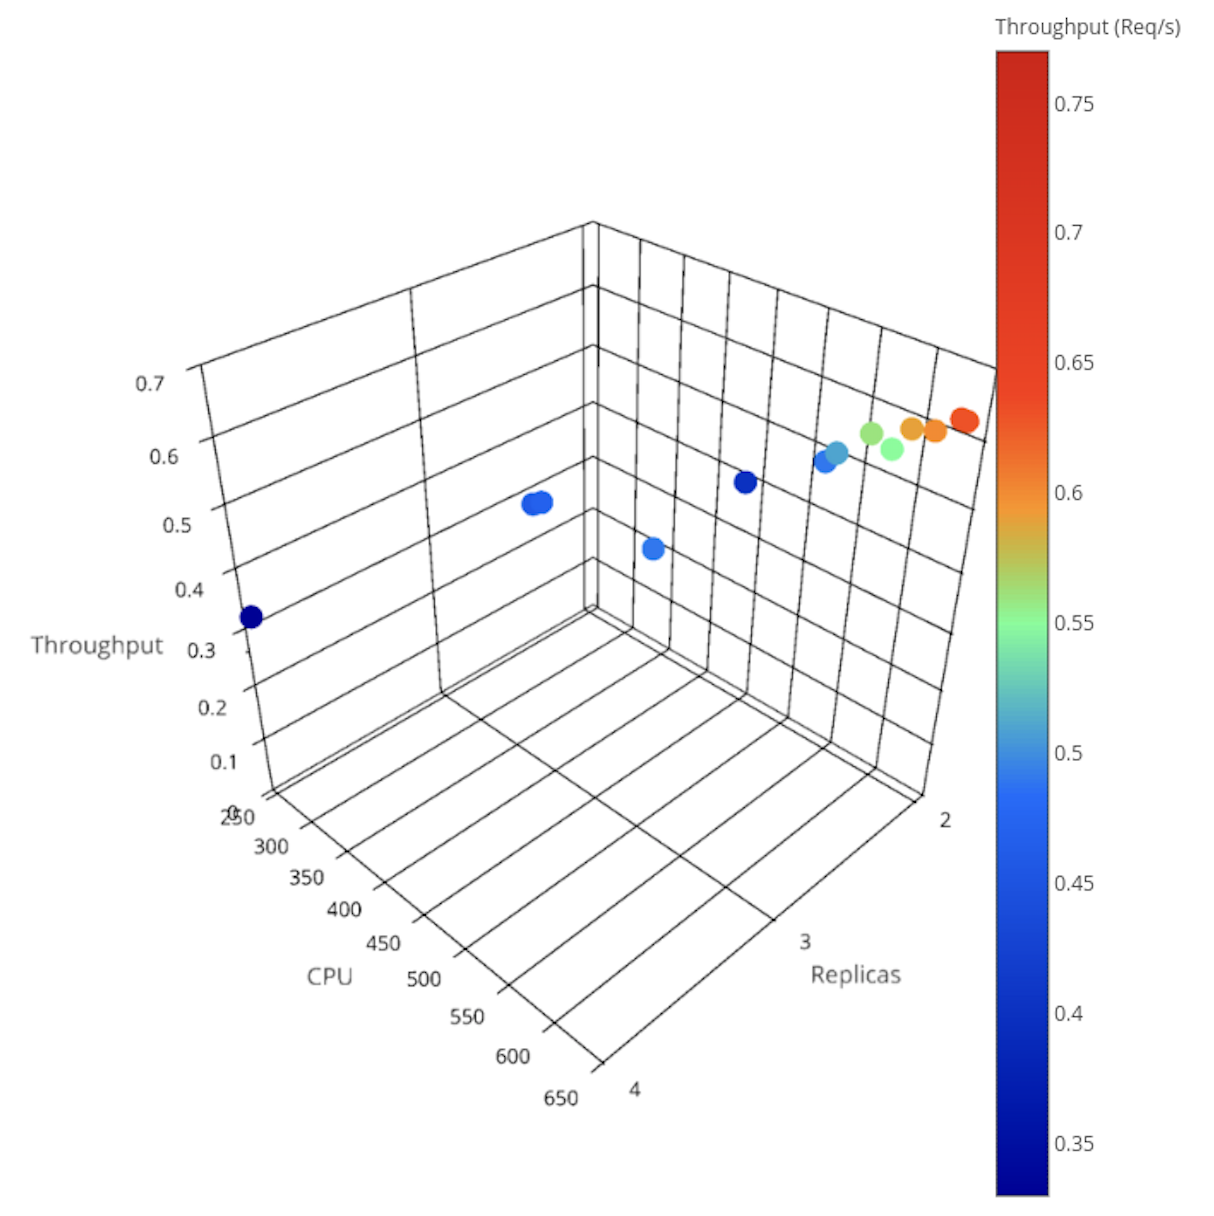
\includegraphics[width=1\textwidth]{chapter-evaluation/plot_2_final.png}
    \caption{Experiment 6: Throughput vs. CPU and replica configuration. }
    \label{fig:exp6-results}
\end{figure}

\begin{table}[H]
\centering
\caption {Experiment 6: Results of k8-resource-optimizer on 15 samples in 5 iterations  Throughput is for job size of 500  tasks.}
\label{tbl:exp6}
\begin{tabular}{lllll}
ITERATION: 1                                  &                                         &                                     &                                                  &                                         \\ \hline
\multicolumn{1}{|l|}{\textbf{workerReplicas}} & \multicolumn{1}{l|}{\textbf{workerCPU}} & \multicolumn{1}{l|}{\textbf{Score}} & \multicolumn{1}{l|}{\textbf{Throughput (Jobs/s)}} & \multicolumn{1}{l|}{\textbf{Total CPU}} \\ \hline
\multicolumn{1}{|l|}{2}                       & \multicolumn{1}{l|}{635}                & \multicolumn{1}{l|}{3.18}           & \multicolumn{1}{l|}{0.63}                        & \multicolumn{1}{l|}{1270}               \\ \hline
\multicolumn{1}{|l|}{4}                       & \multicolumn{1}{l|}{255}                & \multicolumn{1}{l|}{0}              & \multicolumn{1}{l|}{0.33}                        & \multicolumn{1}{l|}{1020}               \\ \hline
\multicolumn{1}{|l|}{3}                       & \multicolumn{1}{l|}{380}                & \multicolumn{1}{l|}{0}              & \multicolumn{1}{l|}{0.46}                        & \multicolumn{1}{l|}{1140}               \\ \hline
                                              &                                         &                                     &                                                  &                                         \\
ITERATION: 2                                  &                                         &                                     &                                                  &                                         \\ \hline
\multicolumn{1}{|l|}{\textbf{workerReplicas}} & \multicolumn{1}{l|}{\textbf{workerCPU}} & \multicolumn{1}{l|}{\textbf{Score}} & \multicolumn{1}{l|}{\textbf{Throughput (Jobs/s)}} & \multicolumn{1}{l|}{\textbf{Total CPU}} \\ \hline
\multicolumn{1}{|l|}{2}                       & \multicolumn{1}{l|}{615}                & \multicolumn{1}{l|}{3.22}           & \multicolumn{1}{l|}{0.6}                         & \multicolumn{1}{l|}{1230}               \\ \hline
\multicolumn{1}{|l|}{2}                       & \multicolumn{1}{l|}{640}                & \multicolumn{1}{l|}{3.17}           & \multicolumn{1}{l|}{0.63}                        & \multicolumn{1}{l|}{1280}               \\ \hline
\multicolumn{1}{|l|}{3}                       & \multicolumn{1}{l|}{390}                & \multicolumn{1}{l|}{0}              & \multicolumn{1}{l|}{0.47}                        & \multicolumn{1}{l|}{1170}               \\ \hline
                                              &                                         &                                     &                                                  &                                         \\
ITERATION: 3                                  &                                         &                                     &                                                  &                                         \\ \hline
\multicolumn{1}{|l|}{\textbf{workerReplicas}} & \multicolumn{1}{l|}{\textbf{workerCPU}} & \multicolumn{1}{l|}{\textbf{Score}} & \multicolumn{1}{l|}{\textbf{Throughput (Jobs/s)}} & \multicolumn{1}{l|}{\textbf{Total CPU}} \\ \hline
\multicolumn{1}{|l|}{3}                       & \multicolumn{1}{l|}{510}                & \multicolumn{1}{l|}{0}              & \multicolumn{1}{l|}{0.49}                        & \multicolumn{1}{l|}{1530}               \\ \hline
\multicolumn{1}{|l|}{2}                       & \multicolumn{1}{l|}{595}                & \multicolumn{1}{l|}{3.26}           & \multicolumn{1}{l|}{0.59}                        & \multicolumn{1}{l|}{1190}               \\ \hline
\multicolumn{1}{|l|}{2}                       & \multicolumn{1}{l|}{440}                & \multicolumn{1}{l|}{0}              & \multicolumn{1}{l|}{0.4}                         & \multicolumn{1}{l|}{880}                \\ \hline
                                              &                                         &                                     &                                                  &                                         \\
ITERATION: 4                                  &                                         &                                     &                                                  &                                         \\ \hline
\multicolumn{1}{|l|}{\textbf{workerReplicas}} & \multicolumn{1}{l|}{\textbf{workerCPU}} & \multicolumn{1}{l|}{\textbf{Score}} & \multicolumn{1}{l|}{\textbf{Throughput (Jobs/s)}} & \multicolumn{1}{l|}{\textbf{Total CPU}} \\ \hline
\multicolumn{1}{|l|}{2}                       & \multicolumn{1}{l|}{580}                & \multicolumn{1}{l|}{3.29}           & \multicolumn{1}{l|}{0.55}                        & \multicolumn{1}{l|}{1160}               \\ \hline
\multicolumn{1}{|l|}{2}                       & \multicolumn{1}{l|}{520}                & \multicolumn{1}{l|}{0}              & \multicolumn{1}{l|}{0.49}                        & \multicolumn{1}{l|}{1040}               \\ \hline
\multicolumn{1}{|l|}{3}                       & \multicolumn{1}{l|}{605}                & \multicolumn{1}{l|}{2.57}           & \multicolumn{1}{l|}{0.75}                        & \multicolumn{1}{l|}{1815}               \\ \hline
                                              &                                         &                                     &                                                  &                                         \\
ITERATION: 5                                  &                                         &                                     &                                                  &                                         \\ \hline
\multicolumn{1}{|l|}{\textbf{workerReplicas}} & \multicolumn{1}{l|}{\textbf{workerCPU}} & \multicolumn{1}{l|}{\textbf{Score}} & \multicolumn{1}{l|}{\textbf{Throughput (Jobs/s)}} & \multicolumn{1}{l|}{\textbf{Total CPU}} \\ \hline
\multicolumn{1}{|l|}{2}                       & \multicolumn{1}{l|}{560}                & \multicolumn{1}{l|}{3.34}           & \multicolumn{1}{l|}{0.56}                        & \multicolumn{1}{l|}{1120}               \\ \hline
\multicolumn{1}{|l|}{2}                       & \multicolumn{1}{l|}{530}                & \multicolumn{1}{l|}{3.42}           & \multicolumn{1}{l|}{0.51}                        & \multicolumn{1}{l|}{1060}               \\ \hline
\multicolumn{1}{|l|}{3}                       & \multicolumn{1}{l|}{590}                & \multicolumn{1}{l|}{2.6}            & \multicolumn{1}{l|}{0.77}                        & \multicolumn{1}{l|}{1770}               \\ \hline
\end{tabular}
\end{table}

\begin{table}[H]
\centering
\caption{Experiment 6: Validation decompositions with fixed amount of worker replicas.  }
\label{tbl:exp6-val}
\begin{tabular}{llll}
ITERATION: 1                                  &                                         &                                     &                                                  \\ \hline
\multicolumn{1}{|l|}{\textbf{workerReplicas}} & \multicolumn{1}{l|}{\textbf{workerCPU}} & \multicolumn{1}{l|}{\textbf{Score}} & \multicolumn{1}{l|}{\textbf{Throughput (Jobs/s)}} \\ \hline
\multicolumn{1}{|l|}{2}                       & \multicolumn{1}{l|}{410}                & \multicolumn{1}{l|}{0}              & \multicolumn{1}{l|}{0.39}                        \\ \hline
\multicolumn{1}{|l|}{2}                       & \multicolumn{1}{l|}{455}                & \multicolumn{1}{l|}{0}              & \multicolumn{1}{l|}{0.43}                        \\ \hline
\multicolumn{1}{|l|}{2}                       & \multicolumn{1}{l|}{505}                & \multicolumn{1}{l|}{0}              & \multicolumn{1}{l|}{0.48}                        \\ \hline
\multicolumn{1}{|l|}{2}                       & \multicolumn{1}{l|}{575}                & \multicolumn{1}{l|}{2.04}           & \multicolumn{1}{l|}{0.54}                        \\ \hline
                                              &                                         &                                     &                                                  \\
ITERATION: 2                                  &                                         &                                     &                                                  \\ \hline
\multicolumn{1}{|l|}{\textbf{workerReplicas}} & \multicolumn{1}{l|}{\textbf{workerCPU}} & \multicolumn{1}{l|}{\textbf{Score}} & \multicolumn{1}{l|}{\textbf{Throughput (Jobs/s)}} \\ \hline
\multicolumn{1}{|l|}{2}                       & \multicolumn{1}{l|}{560}                & \multicolumn{1}{l|}{2.07}           & \multicolumn{1}{l|}{0.54}                        \\ \hline
\multicolumn{1}{|l|}{2}                       & \multicolumn{1}{l|}{570}                & \multicolumn{1}{l|}{2.05}           & \multicolumn{1}{l|}{0.55}                        \\ \hline
\multicolumn{1}{|l|}{2}                       & \multicolumn{1}{l|}{535}                & \multicolumn{1}{l|}{2.12}           & \multicolumn{1}{l|}{0.51}                        \\ \hline
\multicolumn{1}{|l|}{2}                       & \multicolumn{1}{l|}{520}                & \multicolumn{1}{l|}{0}              & \multicolumn{1}{l|}{0.48}                        \\ \hline
                                              &                                         &                                     &                                                  \\
                                              &                                         &                                     &                                                  \\
ITERATION: 1                                  &                                         &                                     &                                                  \\ \hline
\multicolumn{1}{|l|}{\textbf{workerReplicas}} & \multicolumn{1}{l|}{\textbf{workerCPU}} & \multicolumn{1}{l|}{\textbf{Score}} & \multicolumn{1}{l|}{\textbf{Throughput (Jobs/s)}} \\ \hline
\multicolumn{1}{|l|}{3}                       & \multicolumn{1}{l|}{310}                & \multicolumn{1}{l|}{0}              & \multicolumn{1}{l|}{0.36}                        \\ \hline
\multicolumn{1}{|l|}{3}                       & \multicolumn{1}{l|}{355}                & \multicolumn{1}{l|}{0}              & \multicolumn{1}{l|}{0.42}                        \\ \hline
\multicolumn{1}{|l|}{3}                       & \multicolumn{1}{l|}{405}                & \multicolumn{1}{l|}{0}              & \multicolumn{1}{l|}{0.49}                        \\ \hline
\multicolumn{1}{|l|}{3}                       & \multicolumn{1}{l|}{475}                & \multicolumn{1}{l|}{2.05}           & \multicolumn{1}{l|}{0.58}                        \\ \hline
                                              &                                         &                                     &                                                  \\
ITERATION: 2                                  &                                         &                                     &                                                  \\ \hline
\multicolumn{1}{|l|}{\textbf{workerReplicas}} & \multicolumn{1}{l|}{\textbf{workerCPU}} & \multicolumn{1}{l|}{\textbf{Score}} & \multicolumn{1}{l|}{\textbf{Throughput (Jobs/s)}} \\ \hline
\multicolumn{1}{|l|}{3}                       & \multicolumn{1}{l|}{460}                & \multicolumn{1}{l|}{2.09}           & \multicolumn{1}{l|}{0.57}                        \\ \hline
\multicolumn{1}{|l|}{3}                       & \multicolumn{1}{l|}{470}                & \multicolumn{1}{l|}{2.06}           & \multicolumn{1}{l|}{0.58}                        \\ \hline
\multicolumn{1}{|l|}{3}                       & \multicolumn{1}{l|}{435}                & \multicolumn{1}{l|}{2.15}           & \multicolumn{1}{l|}{0.52}                        \\ \hline
\multicolumn{1}{|l|}{3}                       & \multicolumn{1}{l|}{420}                & \multicolumn{1}{l|}{2.19}           & \multicolumn{1}{l|}{0.51}                        \\ \hline
\end{tabular}
\end{table}
\newpage
\section{Summary of experiment results}
In this chapter, an evaluation was presented of the various capabilities of k8-resource-optimizer. Experiment 1 validated the correctness of the employed workload generator. In the remaining experiments, k8-resource-optimizer was evaluated in the following scenarios: single parameter tuning of a single tenant, a mix of homogeneous tenants, a mix of heterogeneous tenants and multiple parameter tuning. In all scenarios, k8-resource-optimizer was capable to produce an acceptable decomposition within the given constraints. Overall, the results are promising for the applicability of auto-tuning for SLA-decomposition in a multi-tenant Kubernetes environment. \\\\
Due to timing constraints, k8-resource-optimizer was not evaluated in the context of tuning multiple components. Results similar to those of multiple parameters are expected in this scenario. This proposed as future work. In addition, future work could include exploration to eliminate unnecessary preliminary backtracking of BestConfig's optimization algorithm and to reduce the runtime of Locust experiments. 

